% !TEX encoding = UTF-8 Unicode
% !TEX root = rapport.tex

\part{Historique de l'intégration des technologies de l'information \ldots}\label{quoi}

\chapter*{Avant-propos~: Technologies \og{}Informatiques\fg{}?}

\begin{minipage}[H]{0.3\linewidth}
  \begin{figure}[H]
  \centering
  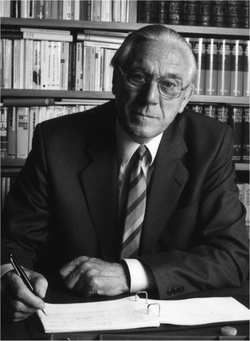
\includegraphics[width=0.8\textwidth]{../resources/illustrations/steinbuch}
  \caption{Karl Steinbuch}
  \end{figure}
\end{minipage}
\begin{minipage}[H]{0.7\linewidth}
Le mot \og{}informatique\fg{} est une concatenation d'\og{}information\fg{} et \og{}automatique\fg{} fait en 1957 par Karl Steinbuch\cite{steinbuch-2005} pour décrire le traitement automatique de l'information.

Depuis le terme a été adopté pour décrire une gamme tellement vaste de sciences, de technologies et de services qu'il a besoin d'être qualifié pour avoir un sens précis.
\vspace{1cm}
\end{minipage}

\begin{coolquote}[Wikipedia\cite{wiki-informatique}]
Les expressions \textbf{science informatique}, \textbf{informatique fondamentale} ou \textbf{informatique théorique} sont utilisées pour désigner sans ambiguïté la science, tandis que \emph{technologies de l'information} ou \textbf{technologies de l'information et de la communication} désignent le secteur industriel et ses produits.
\end{coolquote}

Ici nous utiliserons \textbf{technologies de l'information} pour décrire toute technique permettant de stoquer, de traiter ou de transférer l'information. Cette définition couvre évidemment les algorithmes, structure données et protocoles de communication, mais aussi les langages naturels, l'écriture, et tout outil de réflexion logico-mathématique\ldots

\chapter{Le langage~: protocole de communication}
Avec l'apparition du langage l'Être humain s'est doté d'un outil capable d'exprimer des informations de plus en plus complexes. Environ 6000 langues sont parlés aujourd'hui; les Anthropologues n'ont jamais découvert un peuple démunie d'un langage complexe\cite{linguistics-pinker}. 

Il est difficile de dater l'appararition du langage. L'Homme essaye pourtant depuis des milliers d'années de trouver un \og{}proto-language\fg{}, origine de toute autre, mais sans succès. Dans \og{}L'Enquête\fg{}, l'historien Grecque Hérodote fait référence à une expérience de \og{}privation de langage\fg{} du pharaon Psammétique~I visant à déterminer le langage \og{}par défaut\fg{} de l'Homme\cite{herodote-privation}. 

\begin{minipage}[H]{0.32\linewidth}
  \begin{figure}[H]
  \centering
  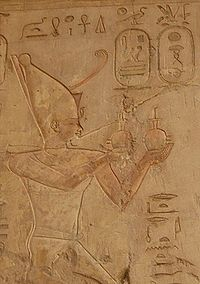
\includegraphics[width=0.8\textwidth]{../resources/illustrations/psamtik-I}
  \caption{Pharaon Psammétique~I}
  \end{figure}
\end{minipage}
\begin{minipage}[H]{0.32\linewidth}
  \begin{figure}[H]
  \centering
  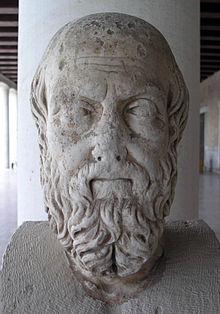
\includegraphics[width=0.8\textwidth]{../resources/illustrations/herodote}
  \caption{Historien Hérodote}
  \end{figure}
\end{minipage}
\begin{minipage}[H]{0.32\linewidth}
  \begin{figure}[H]
  \centering
  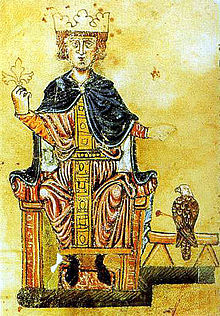
\includegraphics[width=0.8\textwidth]{../resources/illustrations/fred-II}
  \caption{Empereur Frédéric~II}
  \end{figure}
\end{minipage}

\begin{minipage}[H]{0.65\linewidth}
De tels expériences furènt répétés au fil de l'histoire, notamment par l'empereur Frédéric~II de Hohenstaufen, pour qui le résultat fut la mort de ses \og{}cobayes\fg{}\cite{ggcoulton-francis-to-dante}. 

Des exemples plus modernes d'enfants \og{}sauvages\fg{} ont conduits à l'hypothèse de la \og{}période critique\fg{} de Wilder Penfield et Lamar Roberts\cite{penfield2003speech}, popularisé par Eric Lenneberg\cite{lenneberg-crit-period}~: un enfant privé de vocalisations pendant les première années de sa vie sera incapable de bien assimiler le langage par la suite.
\vspace{1cm}
\end{minipage}
\begin{minipage}[H]{0.34\linewidth}
  \begin{figure}[H]
  \centering
  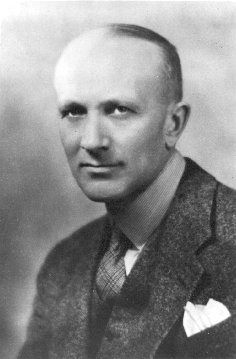
\includegraphics[width=0.8\textwidth]{../resources/illustrations/penfield}
  \caption{Wilder Penfield}
  \end{figure}
\end{minipage}

Peu importe son ou ses origines, le langage est une technologie de l'information primordiale. Il permet un transfert d'informations entre membres d'une société mais aussi, par le bias des traditions orales, un stockage de l'information pendant une durée théoriquement infini. Chez les peuples alettrés une deuxième invention, la structure d'épopée, est souvent utilisé pour faciliter partage et mémorisation des récits sous form de poésies rythmés \cite{havelock-preface-plato}. Notons d'ailleurs que la poésie est toujours utilisé aujourd'hui comme exercise de mémorisation (à l'école) et moyen mnémotechnique (surtout dans la publicité).

\chapter{L'écriture~: mémoire externe}
Si le langage peut être vu comme un instinct plutôt qu'une technologie, ce n'est pas le cas de l'écriture. L'écriture idéographique n'est apparu, il y environ 5000 ans, chez un nombre limité de civilisations. L'écriture alphabétique d'ailleurs semble n'être apparu qu'une seule fois, chez les Cananéens, il y a 3700 ans\cite{linguistics-pinker}. Toute autre écriture alphabétique se serait donc dérivé de celle-ci.
%\gls{Écriture alphabétique~: écriture où chaque symbole correspond à un son vocal.}

En tout cas l'invention permet à un support mort de stoquer un ensemble de données codés sous forme de symboles, donc de repousser d'avantage la frontière de l'espace et du temps. Cette avancé rend presque redondants les techniques de mémorisation lyriques mentionnées ci-dessus. La réaction de ceux qui se sont investies dedans est donc peu surprenant~:


\begin{coolquote}[Platon\cite{plato-phaedrus}]
Elle ne peut produire dans les âmes, en effet, que l’oubli de ce qu’elles  savent en leur faisant négliger la mémoire. Parce qu’ils auront foi dans  l’écriture, c’est par le dehors, par des empreintes étrangères, et non plus du dedans et du fond d’eux-mêmes, que les hommes chercheront à se ressouvenir. 

Tu as trouvé le moyen, non point d’enrichir la mémoire, mais de conserver les souvenirs qu’elle a. Tu donnes à tes disciples la présomption qu’ils ont la science, non la science elle-même. Quand ils auront, en effet, beaucoup appris sans maître, ils s’imagineront devenus très savants, et ils ne seront pour la plupart que des ignorants de commerce incommode, des savants imaginaires au lieu de vrais savants.
\end{coolquote}

\begin{minipage}[H]{0.49\linewidth}
  \begin{figure}[H]
  \centering
  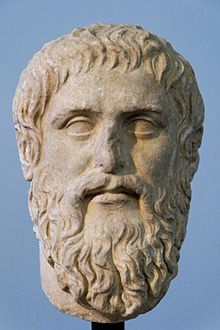
\includegraphics[height=0.15\paperheight]{../resources/illustrations/plato2}
  \caption{Plato}
  \end{figure}
\end{minipage}
\begin{minipage}[H]{0.49\linewidth}
  \begin{figure}[H]
  \centering
  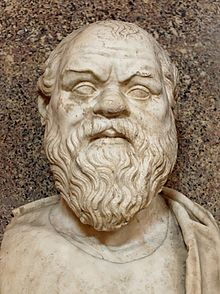
\includegraphics[height=0.15\paperheight]{../resources/illustrations/socrates}
  \caption{Socrates}
  \end{figure}
\end{minipage}

\begin{minipage}[H]{0.3\linewidth}
  \begin{figure}[H]
  \centering
  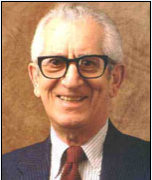
\includegraphics[width=0.8\textwidth]{../resources/illustrations/bloom_face}
  \caption{Benjamin Bloom}
  \end{figure}
\end{minipage}
\begin{minipage}[H]{0.69\linewidth}
Cette critique fait à travers un dialogue entre Socrates et Phaedrus, suggère que l'écriture, en plus de nuire à la mémoire, limite son lecteur à ce que la taxonomie de Bloom\cite{tax-bloom} appelerait \textbf{connaître} à la différence de \textbf{comprendre}, \textbf{appliquer} et cetera. 

Pour Platon une conaissance ne peut être transféré correctement sans être assimilé, or le papier, si bien soit-il capable de stoquer des propos, est incapable de les comprendre ou de les défendre.
\vspace{1cm}
\end{minipage}

Il ne faut pas oublier, cependant, que Platon était un professeur dont la pédagogie se repossait sur le dialogue et non la lecture. Il n'est donc pas un interlocuteur très objective. Notons également avec ironie que si nous connaissons Platon c'est grâce à l'écriture, et si nous confondons Socrates avec lui c'est que ce dernier n'a laissé aucune trace écrite.

Celà étant, les critiques de Platon restent pertinentes aujourd'hui, voir le deviennent d'autant plus~: la consultation d'informations est maintenant tellement facile que la mémorisation semble suranné, mais il y une distinction importante à faire entre éfleurer un propos et l'assimiler.

Quand nous nous approprions véritablement d'un propos il devient bien plus qu'une copie supplémentaire redondant~: l'idée nous appartient, nous change et est changé pour nous\ldots

\chapter{L'imprimerie~: reproduction des données}

Pendant le Moyen Âge le centre intellectuelle du monde quitte l'Europe pour le Moyen Orient


\chapter{L'horloge maritime~: calcul automatique}
Nous pourrions remplir un rapport tout entier s'il était question d'énumérer les apports de l'outil logico-mathématique, donc nous nous limiterons à l'exemple pertinente des tables de logarithmes. Les logarithmes de Napier, introduits en 1614 dans son oeuvre \og{}Mirifici Logarithmorum Canonis Descriptio\fg{}, furent un outil abstrait visant à simplifier des calculs complexes. Les tables de logarithmes sont très vite devenus indispensables pour tout mathématicien, ingénieur, navigateur ou scientifique.

\begin{coolquote}[Pierre-Simon Laplace\cite{history-of-astronomy}]
[Les logarithmes sont] un artifice admirable qui, en réduisant à quelques jours un travail de plusieurs mois, double la durée de vie de l'astronome, et lui épargne les erreurs et le dégoût : plaies inséparables des longs calculs.
\end{coolquote}

\begin{minipage}[H]{0.49\linewidth}
  \begin{figure}[H]
  \centering
  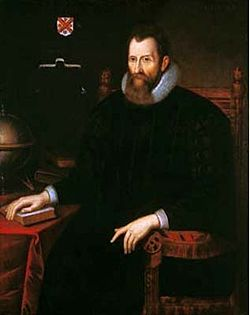
\includegraphics[height=0.15\paperheight]{../resources/illustrations/napier}
  \caption{John Napier}
  \end{figure}
\end{minipage}
\begin{minipage}[H]{0.49\linewidth}
  \begin{figure}[H]
  \centering
  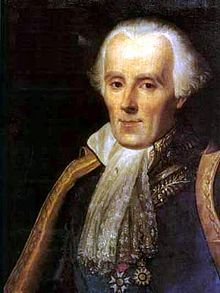
\includegraphics[height=0.15\paperheight]{../resources/illustrations/laplace}
  \caption{Pierre-Simon Laplace}
  \end{figure}
\end{minipage}
L'utilisation des logarithmes se repose sur des tables de précalcule tels l'\oe{}uvre de 1617 d'Henri Briggs. Muni d'une telle table la multiplication de deux nombres, par exemple, devient triviale~:

\begin{eqnarray}
                    &x            &= 2.16\times{8.13}              \nonumber \\
        \implies{}  &\log{x}      &= \log{2.16}+\log{8.13}         \nonumber \\
                    &             &= 0.3344548 + 0.9100905         \nonumber \\
                    &             &= 1.2445443                     \nonumber \\
        \implies{}  &x            &\approx{17.56}                   \nonumber \\
\end{eqnarray}

La table nous donne directement $\log{2.16}$ et $\log{8.13}$, et nous pouvoir également lire que le logarithme le plus proche est $log{17.56} = 1.2445245$. Nous en déduisons donc en quelques instants $2.16\times{8.13} \approx{17.56}$, ce qui n'est pas loin de de la vraie valeur $2.16\times{8.13}={17.5608}$. Il s'agit en somme d'un algorithme approximatif à base de tables de pré-calcule~: notons que de tels algorithmes existent depuis les Babyloniens\cite{robson-math}.

Laplace parle de l'astronome, car il s'agit de l'époque des grandes découvertes~: pour naviger on ne peut s'en passer des almanachs astrales et des algorithmes de navigation astronomique qui se reposaient dessus. Cependant si la latitude peut se calculer grace à l'hauteur perçu du soleil, la longitude est déterminé à partir de la conaissance de l'heure exacte en un endroit précis~: $4$ minutes de décalage correspond à une différence de longitude de $1^{\circ}$.  

\begin{minipage}[H]{0.59\linewidth}
  \begin{figure}[H]
  \centering
  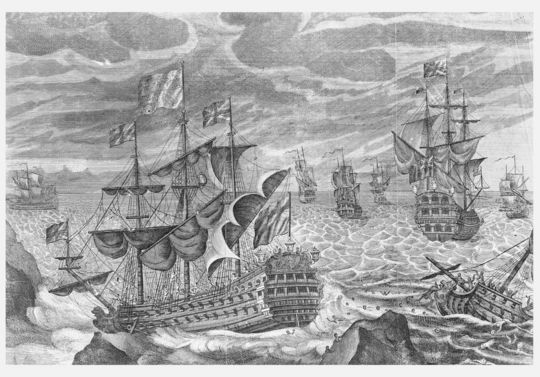
\includegraphics[width=0.8\textwidth]{../resources/illustrations/scilly1707}
  \caption{Désastre naval de Sorlingues}
  \end{figure}
\end{minipage}
\begin{minipage}[H]{0.39\linewidth}
En 1714, après la perte en 1707 de 1,400 hommes et 4 navires à Sorlingues suite à un mauvais calcul de position, le parlement Britannique offre un prix de \pounds{20,000} à celui qui saura déterminer, avec une erreur maximum de 56 km, la longitude d'un navire en mer\cite{longitude}. 
%\vspace{1cm}
\end{minipage}

Entre en jeu le charpentier John Harrison, horlogier autodidacte qui construit 1736 la première horloge capable de fonctionner en voyage maritime, suivi d'autres toujours plus compactes et toujours plus précises. Cette invention fut cependant rejeté par l'orthodoxie académique de l'époque, qui voulaient impérativement une solution algorithmique-astrologique tel la méthode des distances lunaires, introduite en Angleterre en 1674 et perfectionnée par Nevil Maskelyne en 1767\cite{history-longitude}.

\begin{minipage}[H]{0.49\linewidth}
  \begin{figure}[H]
  \centering
  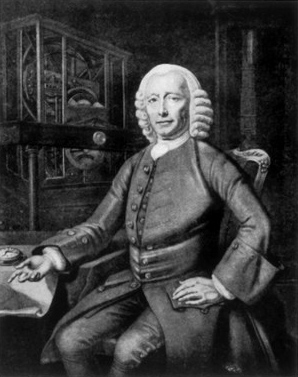
\includegraphics[height=0.15\paperheight]{../resources/illustrations/jharrison}
  \caption{John Harrison}
  \end{figure}
\end{minipage}
\begin{minipage}[H]{0.49\linewidth}
  \begin{figure}[H]
  \centering
  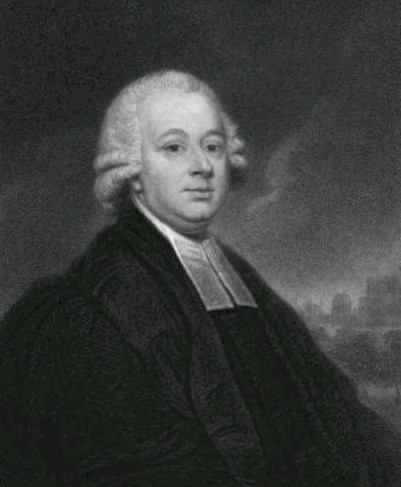
\includegraphics[height=0.15\paperheight]{../resources/illustrations/maskelyne}
  \caption{Nevil Maskelyne}
  \end{figure}
\end{minipage}

Harrison aura besoin d'attendre 1773 pour recevoir une prime réduite de \pounds{8,750}, et ne sera pas officiellement reconnu comme gagnant.

Pourqui ce rejet? Il s'agit d'un Homme ayant conçu un \og{}oracle\fg{} capable de résoudre le problème pour lui et non pas, distinction importante, une méthode lui permettant de le résoudre lui-même. L'informaticien devient alors prêtre d'un Dieu-machine plutôt que mathématicien-philosophe~: proposition controverse. Ce débat, entre ingénierie et science, trouve son écho aujourd'hui autour de l'apprentissage automatique~: nous pouvons concevoir des machines capable de reconaître des visages, sans comprendre pour autant comment fonctionne cette reconaissance. 

Notons également que de nos jours les algorithmes de calcul à base de tables logarithmiques ne sont même pas introduites à l'école~: la popularisation de calculatrices électroniques aux année 1970 leur ont rendus désuets, de même que l'écriture rend inutile l'épopée. Si des machines à calculer tels le Boulier existent depuis environ 4000 ans, ceux-ci ne sont véritablement que des supports mémoires~: c'est l'étudiant qui applique l'algorithme permettant de calculer le résultat désiré. 

Nous pouvions nous dire que le calcul mentale n'a peu d'importance maintenant que les machines à calcul sont omniprésent, mais la foi en une machine n'est pas moins dangereux que la foi en générale, s'il est sans mesure. 


\chapter{Les technologies du \og{}Broadcast\fg{}~: presse, radio, télévision, internet, \ldots}


%\subsection{Les tournant majeur des technologies de l'information}
//@? Comment introduire la notion de document ?

Les technologies de l'information n'ont eu de cesse de repousser les limites de
la propagation de l'information, 

Avec l'arrivée de l'imprimante, l'Homme est désormais capable de copier
rapidement une information pour la \emph{diffuser}. (Apparition d'une sorte
de broadcast)

Avec le téléphone, l'Homme peut désormais échanger \emph{en tant réelle} une 
information avec une autre personne \og{}~n'importe où~\fg{} dans le monde.

La télévision permet non seulement de faire de même avec des images, mais elle,
ou plutôt son usage, permet bien plus. Elle permet de préformater un document pour ensuite le
diffuser et éventuellement le rediffuser à l'attention d'un public nombreux et
hétérogène tel que l'on peut le faire avec un livre.

Puis vint Internet \og{}~International Network~\fg{}, en vrac: n'importe qui
peut diffuser un document pour un coup très faible, une quantité astronomique
de documents accessibles, Internet se présente comme un méta-outil et offre de
nombreux outils de communication (Mail, Forum, chat, VoIP, conférence, etc...)

\section{en vrac}



Depuis les années 90: internet, outil pour tricher?
%--BROKEN \url{http://www.apsq.org/sautquantique/doss/d-tricherie.html/}

\ldots

\chapter{\ldots dans la société}

La notion de nation est-elle pertinente dans un monde connecté par
internet~?

"The Big Switch: Rewiring the World from Edison to Google" 
 \url{http://www.nicholasgcarr.com/bigswitch/}
 
\begin{coolquote}[Mark Zuckerberg\cite{zuckerberg-privacy-guardian}]
"People have really gotten comfortable not only sharing more information and different kinds, but more openly and with more people," he said. "That social norm is just something that has evolved over time."
\end{coolquote}

Nous perdons notre confidentialité de l'intime. Pour Google, Facebook, etc, 
ce n'est pas un problème: ceux qui n'ont rien à cacher n'ont pas à se soucier. Nous
pouvons cependant noter qu'ils ont intérêt à penser ainsi [j'arrive pas à 
trouver l'article qui en parle]. Le voyeurisme de la télé-réalité montre 
que ce phénomène est de Zeitgeist (esprit de l'époque): nous nous soucions 
moins, par exemple, de qui nous entend parler lors de nos
conversations depuis un téléphone portable.

Les réseaux sociaux permettent un exhibitionnisme, et ceci conduit au 
narcissisme:
http://www.guardian.co.uk/technology/2012/mar/17/facebook-dark-side-study-aggressive-narcissism 
[WHY U NO GIVE ME LINK TO ORIGINAL ARTICLE!]

"The Spy in the Coffee Machine: The End of Privacy As We Know It"
 \url{http://eprints.soton.ac.uk/265683/}

En Février 2010 Eben Moglen lance la notion de "Freedom Box" pour faire face à
la centralisation progressive du web. C'est d'ailleurs sa présentation qui fut
l'amorce du projet Diaspora, visant à créer une plateforme sociale décentralisé 
respectant la confidentialité de ses usagers. 

\section{\ldots par les individus}


